% Inbuilt themes in beamer

\documentclass[aspectratio=169]{beamer}
\usepackage[export]{adjustbox}
\usepackage{xcolor}

\definecolor{darkred}{RGB}{176, 31, 36}
\definecolor{darkgreen}{RGB}{44, 95, 47}

\usepackage{listings}
\usepackage{booktabs}
\usepackage{graphicx}

% Title page details: 
\title{Tema 3.3: Transformers}
\subtitle{Mecanismos de atención}

% Theme choice:
\usetheme{Madrid}
\usecolortheme{seagull}
\useinnertheme{circles}

\author{Pablo Pérez Núñez}
 
\setbeamertemplate{navigation symbols}{}
\setbeamertemplate{author}{}

% Ajusta las dimensiones de la diapositiva

\setbeamertemplate{blocks}[rounded][shadow=false]
% \setbeamertemplate{blocks}[default]
\definecolor{myblue}{RGB}{27, 122, 194}
\definecolor{lightblue}{RGB}{55, 150, 225}
\definecolor{lightbluetwo}{RGB}{164, 209, 242}

\setbeamercolor{block title}{bg=lightblue,fg=white}
\setbeamercolor{block body}{bg=lightbluetwo,fg=black}

\setbeamercolor{title}{fg=white, bg =lightblue}
\setbeamercolor{frametitle}{fg=white, bg = lightblue}

\setbeamercolor*{palette secondary}{fg=white,bg=lightblue}

\defbeamertemplate*{footline}{infolines}
{
  \leavevmode%
  \hbox{%
  \begin{beamercolorbox}[wd=\paperwidth,ht=2.25ex,dp=1ex,left]{title in head/foot}%
    \hspace*{2ex} \usebeamerfont{title in head/foot}\insertshorttitle \ - \insertsubtitle
  \end{beamercolorbox}
  % \begin{beamercolorbox}[wd=.25\paperwidth,ht=2.25ex,dp=1ex,right]{date in head/foot}%
  %   \usebeamerfont{date in head/foot}\hspace*{2em}
  %   \insertframenumber{} / \inserttotalframenumber\hspace*{2ex} 
  %\end{beamercolorbox}
  }%
  \vskip0pt%
}

\setbeamertemplate{title page}{
  \centering
  % \usefonttheme{serif}
  \begin{minipage}{0.95\textwidth} % Ajustar el ancho según sea necesario

    \vspace{1em}
    {\color{myblue}\rule{\linewidth}{2pt}\par}
    \vspace{.5cm}
    {\bfseries \huge \textcolor{myblue}{\inserttitle}\par }
    \vspace{1em}
    {\bfseries \LARGE \textcolor{myblue}{\insertsubtitle}\par }
      
    \vspace{2.5em}

    \begin{columns}
      \column{0.6\textwidth}
      \vspace{6em}\\
      {\bfseries \large \textcolor{myblue}{Aprendizaje profundo / Deep Learning}} \\
      \vspace{1em}
      {\textcolor{myblue}{\insertauthor}}
      \column{0.4\textwidth}
      \vfill
      \centering
      
\includegraphics[height=4.5em]{imgs/LogoAEPIA.pdf} \\
      \vspace{1em}
      
\includegraphics[height=2.5em]{imgs/UIMP.png}
    \end{columns}

    \vspace{1em}

    {\color{myblue}\rule{\linewidth}{.5pt}\par}

  \end{minipage}
    

  %  \usefonttheme{default}
}

% Define the template for section slides
\AtBeginSection[]{
  \begin{frame}
    \vfill
    \LARGE\insertsectionhead\par
    {\color{myblue}\rule{\linewidth}{1pt}\par}
    \vfill
  \end{frame}
}
 

% MIS COSAS --------------------------------
% Bloque con margen inferior
\newenvironment{blockm}[1]{%
  \begin{block}{\textbf{#1}}%
  }{%
  \end{block}%
  \vspace{1em}%
}
% Dos imágenes
\newcommand{\twoimages}[3]{%
  \begin{columns}
    \begin{column}{0.5\textwidth}
      \centering
      \includegraphics[width=#3\textwidth]{#1}
    \end{column}
    \begin{column}{0.5\textwidth}
      \centering
      \includegraphics[width=#3\textwidth]{#2}
    \end{column}
  \end{columns}
}

% Comando para mostrar el título de la subsección al inicio de cada nueva subsección
\AtBeginSubsection[]
{
  \begin{frame}
    \vfill
    \small\insertsectionhead\par
    {\color{myblue}\rule{\linewidth}{1pt}\par}
	\LARGE\insertsubsectionhead\par
    \vfill
  \end{frame}
}

% ------------------------------------------

\begin{document}

% Title page frame
\begin{frame}[plain]
	\titlepage 
\end{frame}

\logo{}

\begin{frame}{Introducción}
  \begin{blockm}{Motivación}
    Muchas tareas no necesitan de toda la entrada para predecir la salida.
  \end{blockm}
  \textbf{Ejemplo:} Predecir la clase de una imagen.
  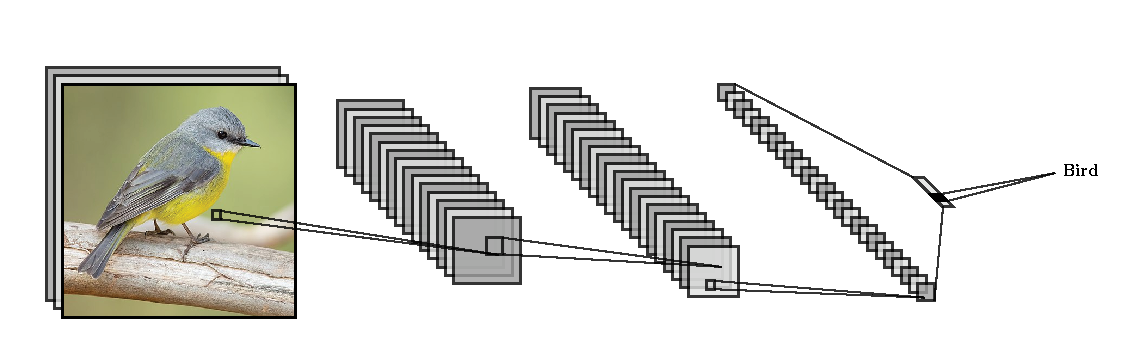
\includegraphics[width=\textwidth, center]{imgs/tema4/att/EX1.1.pdf}
\end{frame}

\begin{frame}{Introducción}
  \begin{blockm}{Motivación}
    Muchas tareas no necesitan de toda la entrada para predecir la salida.
  \end{blockm}
  \textbf{Ejemplo:} Predecir la clase de una imagen.
  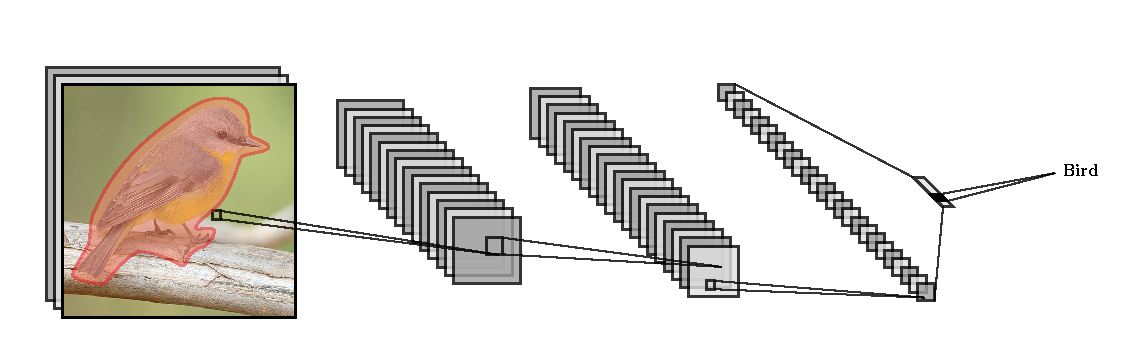
\includegraphics[width=\textwidth, center]{imgs/tema4/att/EX1.2.pdf}
\end{frame}

\begin{frame}{Introducción}
  \begin{blockm}{Motivación}
    Muchas tareas no necesitan de toda la entrada para predecir la salida.
  \end{blockm}
  \textbf{Ejemplo:} Transformar audio en texto.
  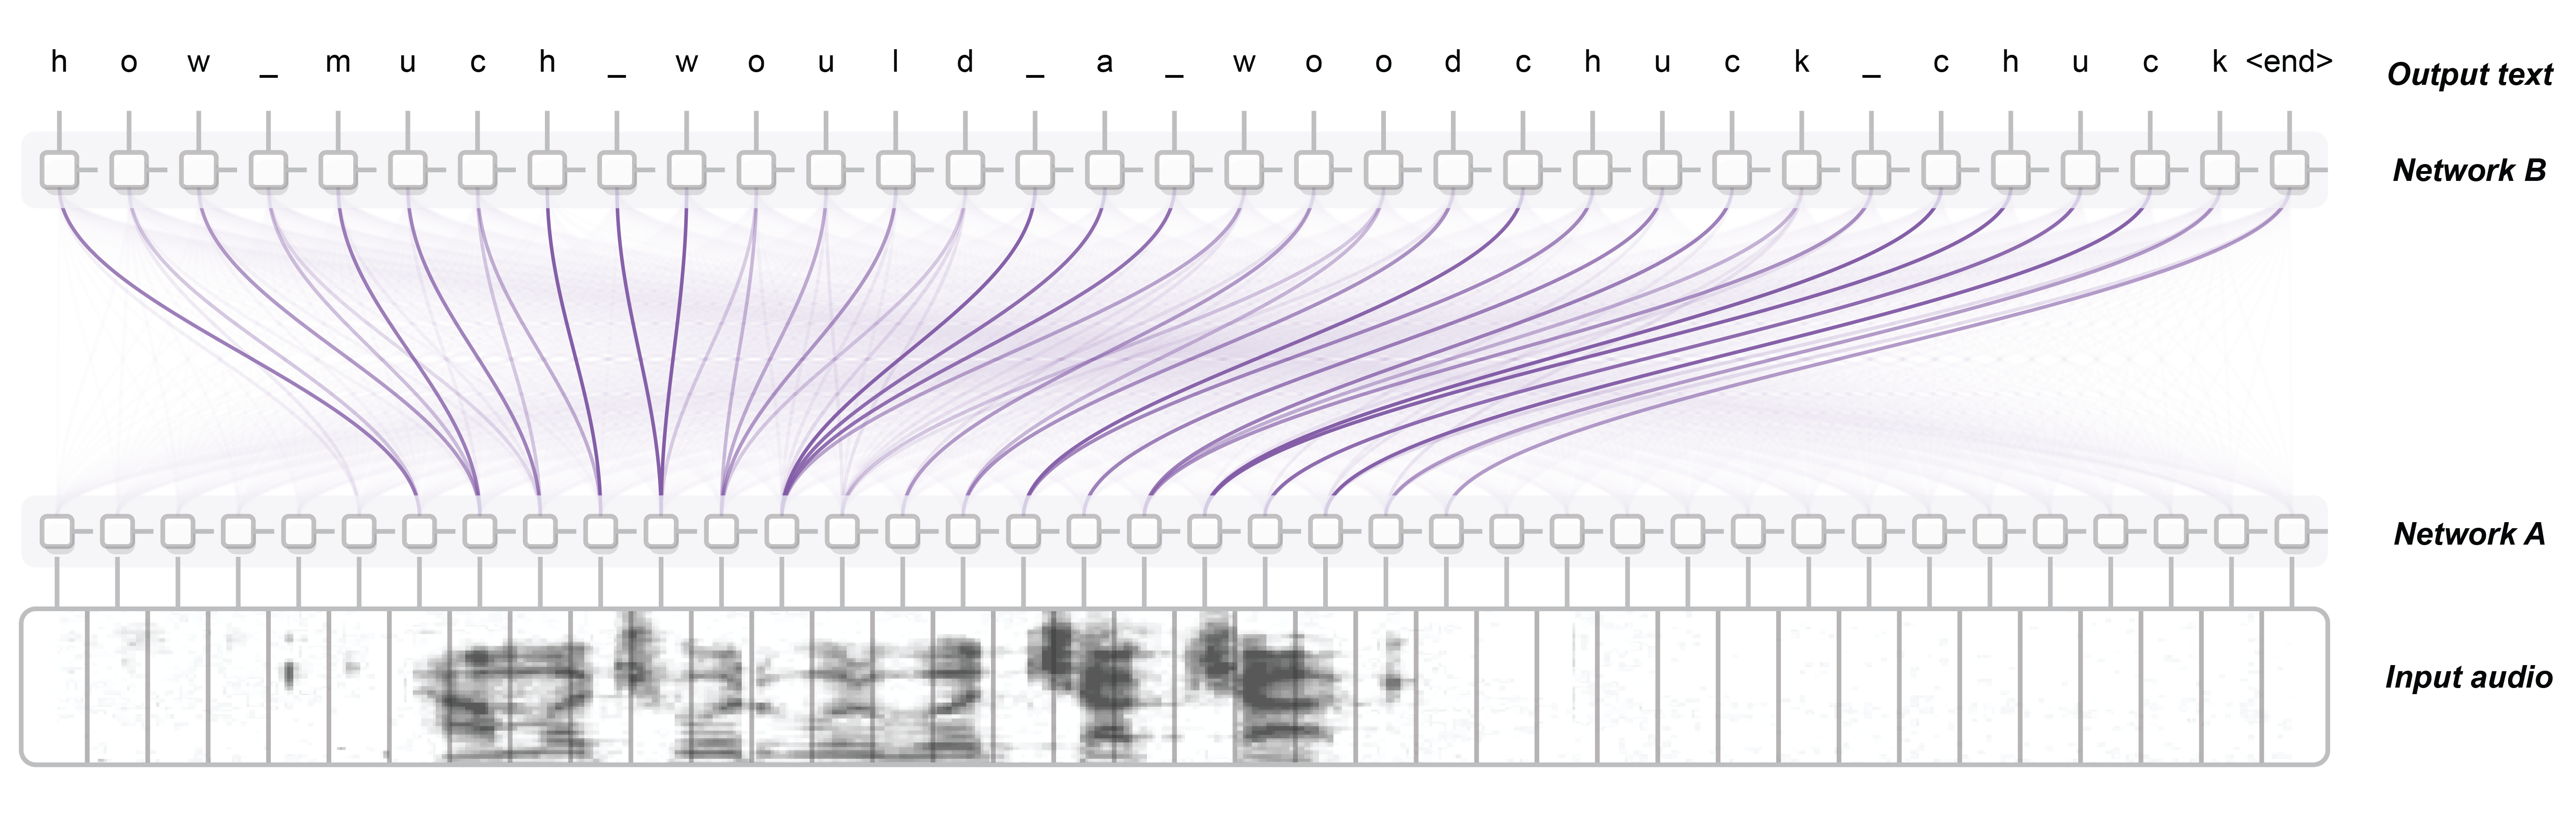
\includegraphics[width=\textwidth, center]{imgs/tema4/att/EX2.png}
\end{frame}

\begin{frame}{Introducción}
  \begin{blockm}{Motivación}
    Muchas tareas no necesitan de toda la entrada para predecir la salida.
  \end{blockm}
  \textbf{Ejemplo:} Traducir entre idiomas.
  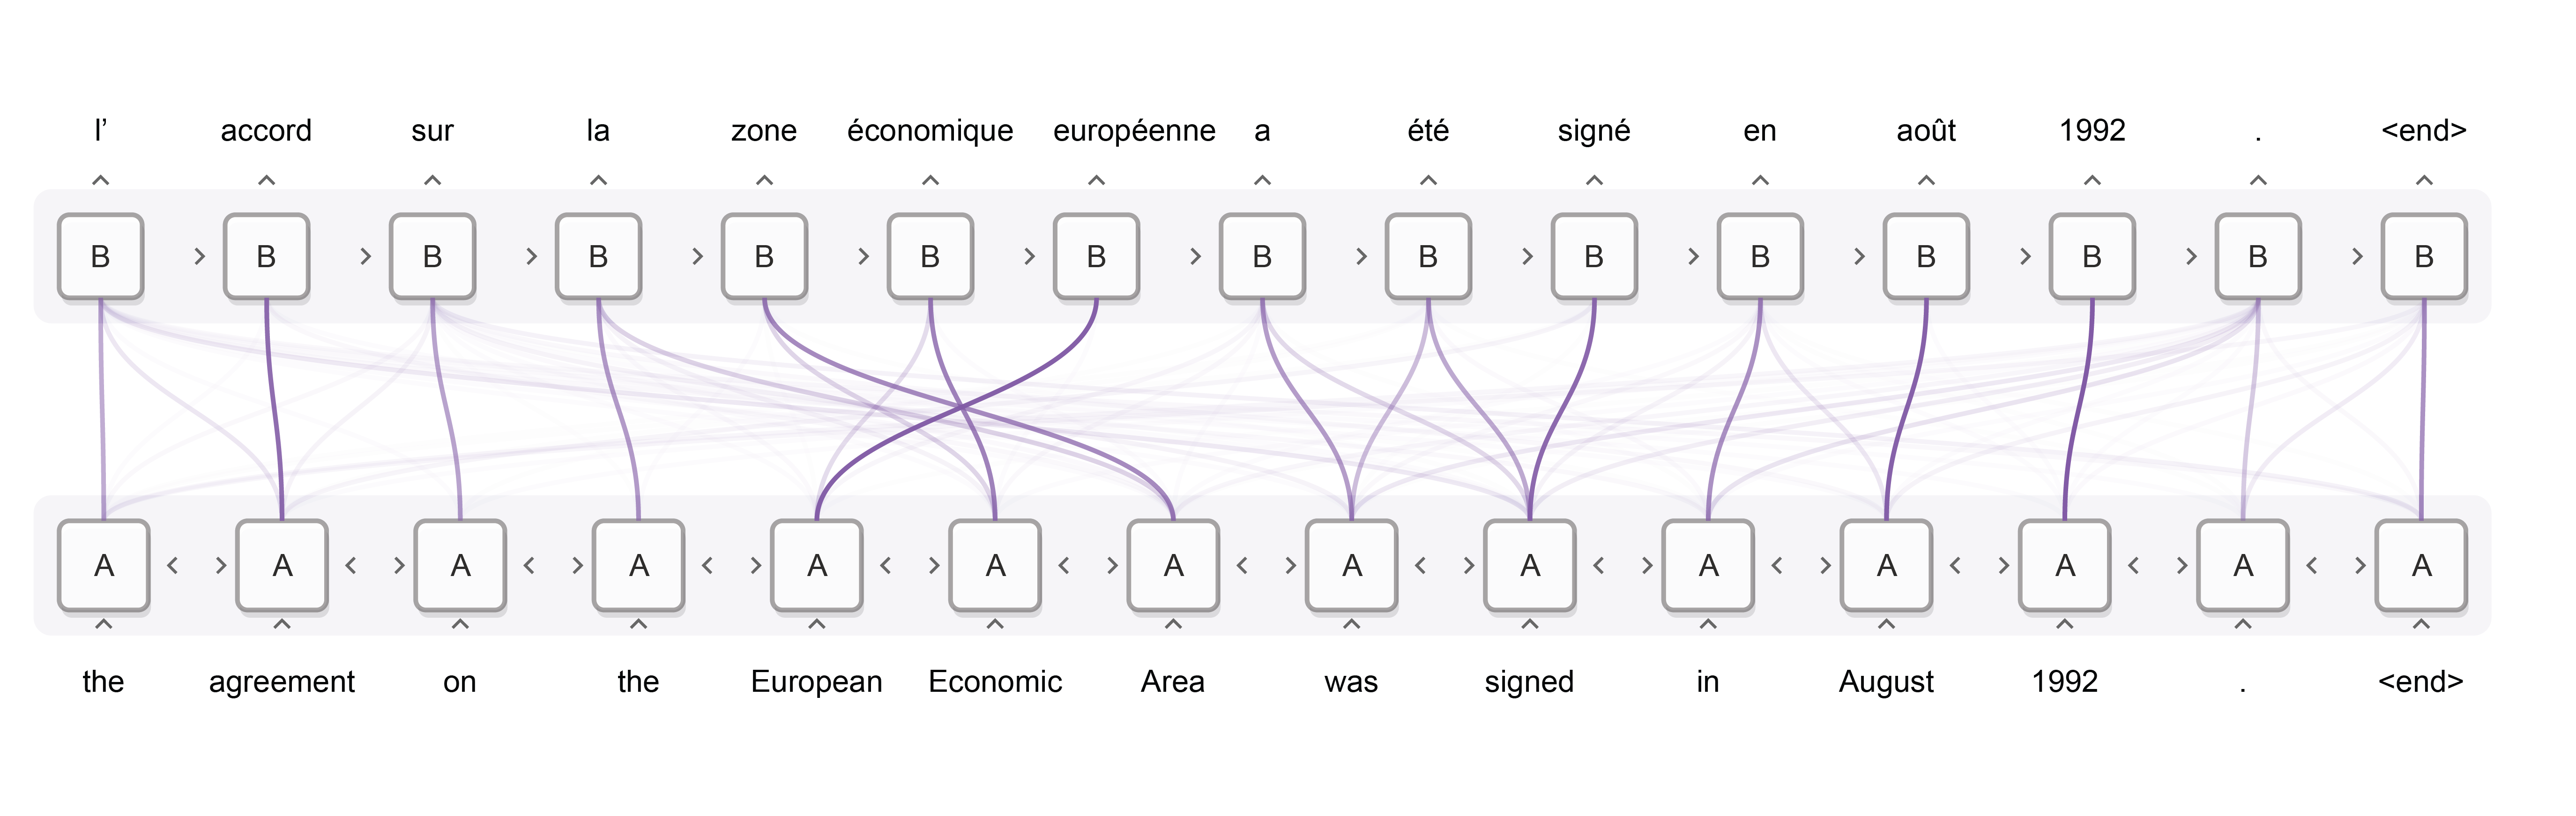
\includegraphics[width=\textwidth, center]{imgs/tema4/att/EX3.png}
\end{frame}

\begin{frame}{Introducción}
  \begin{blockm}{Motivación}
    En tareas de Secuencia a Secuencia, las RNN condensan toda la información de la entrada en un único elemento. No es la mejor opción, sobre todo en largas secuencias. 
  \end{blockm}
  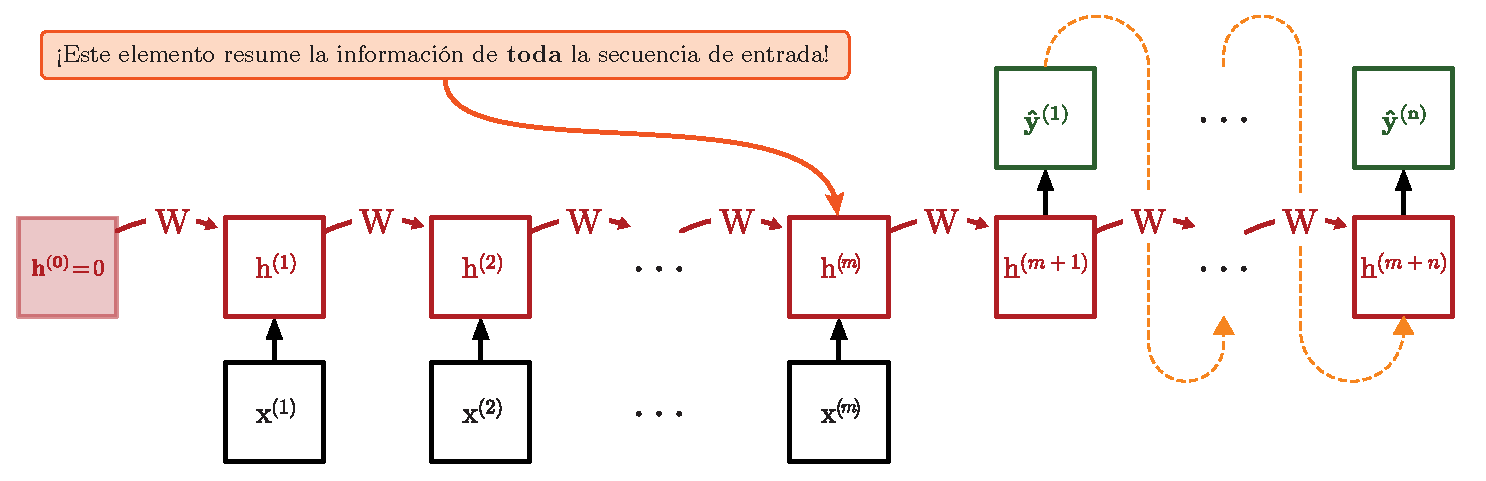
\includegraphics[width=.95\textwidth, center]{imgs/tema4/att/Seq2Seq RNN.pdf}
\end{frame}

\begin{frame}{Introducción}
  \textbf{En este contexto surgen los \emph{Transformers}\footnote{Attention is all you need, Ashish Vaswani et al}}.\\
  \vspace{.5cm}
  Esta nueva arquitectura:
  \begin{itemize}
    \item Mejora la eficiencia computacional de las RNN.
    \item Permite al modelo centrarse en partes concretas de la entrada para predecir la salida.
    \item Soluciona el problema de la memoria corto-placista de las RNN:
    \begin{itemize}
      \item Permiten asociar palabras en una secuencia aunque estén muy separadas entre sí.
    \end{itemize}
  \end{itemize}

\end{frame}

\subsection{Attention mechanisms}

\begin{frame}{Attention mechanisms}
  Antes de comenzar a hablar de \emph{Transformers}, es necesario entender el funcionamiento de su componente principal, los \textbf{attention mechanisms}.
  \vspace{.3cm}
  \begin{blockm}{Definición}
    Los mecanismos de atención seleccionan que elementos de la(s) secuencia(s) de entrada son más importantes para predecir la secuencia salida.
  \end{blockm}
  \vspace{.3cm}

  Detalles:
  \begin{itemize}
    \item  La \textbf{entrada} de estos mecanismos espera \textbf{una o varias secuencias de datos}.
    \item  Dentro de los \emph{Transformers} se utilizan la llamada \emph{Self-attention} pero, como verás a continuación, existen muchas otras variaciones.
  \end{itemize}

\end{frame}

\begin{frame}{Variaciones}
  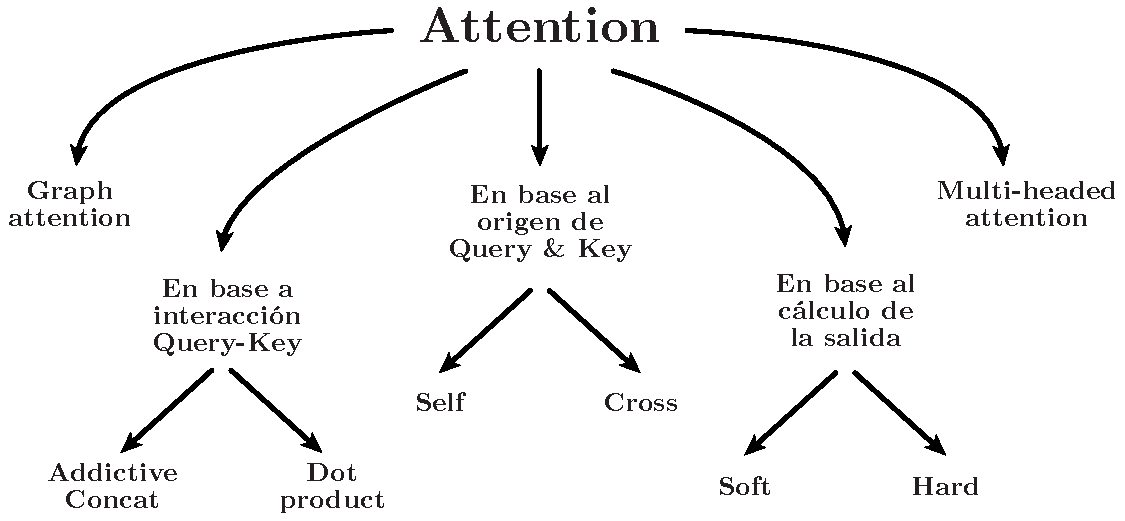
\includegraphics[width=.85\textwidth, center]{imgs/tema4/att/AttOutline.pdf}
\end{frame}

\begin{frame}{Variaciones}
  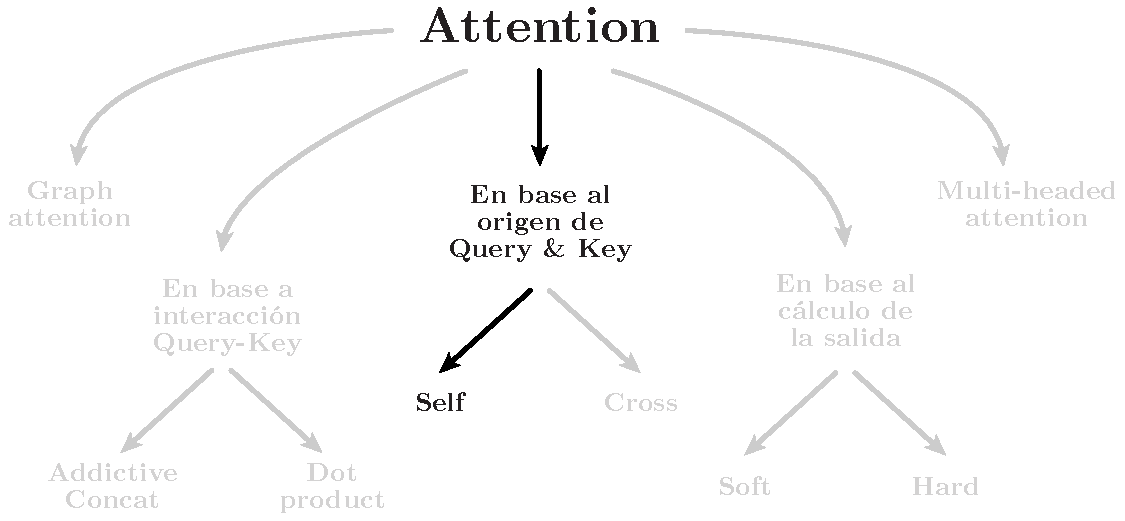
\includegraphics[width=.85\textwidth, center]{imgs/tema4/att/AttOutline self.pdf}
\end{frame}

\subsubsection{Self-attention}

\begin{frame}{Self-attention}

  Este método requiere de los siguientes elementos:
  \begin{itemize}
    \item \textbf{Secuencia de entrada:} $ \mathbf{x}_{1}, \mathbf{x}_{2}, \ldots, \mathbf{x}_{t} $
    \item \textbf{Secuencia de salida:} $ \mathbf{y}_{1}, \mathbf{y}_{2}, \ldots, \mathbf{y}_{t} $
    \item Misma dimensión $ k $ para todos los vectores.
  \end{itemize}

  \vspace{.3cm}

  \begin{block}{}
    Para producir cada vector $ \mathbf{y}_i $ de la secuencia de salida, simplemente se obtiene la media ponderada de las entradas.
  \end{block}

  \begin{equation*}
    \mathbf{y}_{i} = \sum_{j} w_{ij} \mathbf{x}_{j}     
  \end{equation*}
  Donde la $j$ recorre toda la secuencia y la suma de todos los $w_{\cdot j}$ es igual a 1. 
\end{frame}

\begin{frame}{Self-attention}
  \begin{block}{}
    El peso $ w_{i, j} $ \textbf{no es un parámetro}, como en una DNN, se deriva de una función sobre $ \mathbf{x}_{i} $ y $ \mathbf{x}_{j} $.
  \end{block}
  \vspace{.3cm}

  La opción más sencilla para esta función es el \textbf{producto escalar}:
  \begin{equation*}
    w^{'}_{ij} = \left \langle {\mathbf{x}_{i}}^{T}, \mathbf{x}_{j} \right \rangle
  \end{equation*}

  \begin{block}{}
    El peso representa la importancia de cada elemento de la entrada para el elemento actual. 
  \end{block}
  \vspace{.3cm}

  \begin{itemize}
    \item Nótese que $ \mathbf{x}_{i} $ es el vector de entrada en la misma posición que el vector de salida actual.
    \item Para $ \mathbf{y}_{i+1} $, obtenemos una serie completamente nueva de productos escalares y una suma ponderada diferente.
  \end{itemize}

\end{frame}

\begin{frame}{Self-attention}

  El producto escalar anterior nos da valores entre $[-\inf, \inf]$.
  \begin{itemize}
    \item Para obtener valores entre $[0,1]$, aplicamos una \textit{softmax}.
    \item De esta forma, para cada $i$, todos los $j$ pesos sumarán 1.
  \end{itemize}

  \vspace{.3cm}
  Finalmente: 
  \begin{equation*}
    w_{ij} = \frac{\text{exp}\ w^{'}_{ij}}{\sum_{j} \text{exp}\ w^{'}_{ij}}
  \end{equation*}

\end{frame}

\begin{frame}{Self-attention}

  De forma gráfica (softmax omitida por simplicidad):\\
  \vspace{.3cm}
  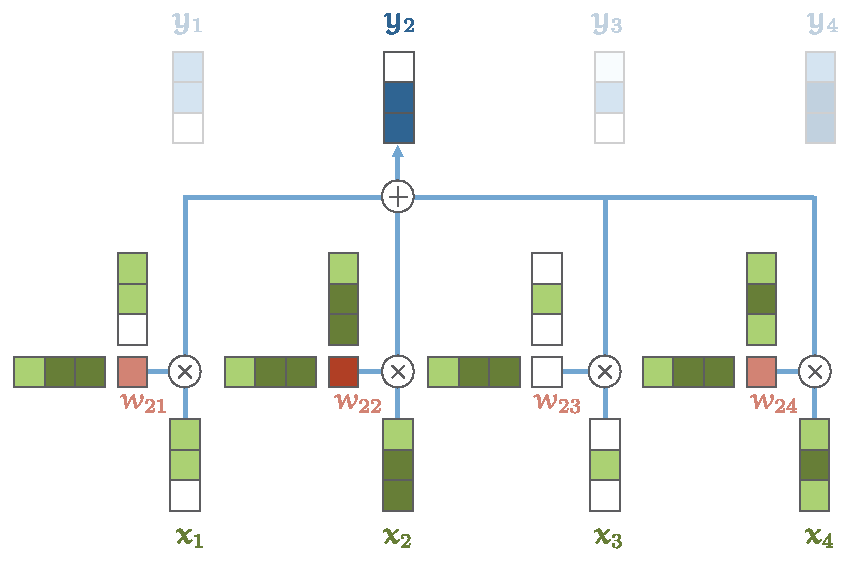
\includegraphics[width=.65\textwidth, center]{imgs/tema4/att/SAT_basic.pdf}

\end{frame}

\begin{frame}{Self-attention}

  Realizando este proceso para todos los $\mathbf{x}_{i}$ obtendremos una matriz de pesos como la representada en la figura.\\

  \begin{columns}
    
    \begin{column}{0.5\textwidth}
      Nótese que:
      \begin{itemize}
        \item Esta matriz se conoce como \textbf{matriz de atención}.
        \item Tras aplicar la softmax, todas las filas de esta matriz suman 1.
        \item A causa de esta softmax, la matriz no tiene por que ser simétrica. 
      \end{itemize}
    \end{column}

    \begin{column}{0.5\textwidth}
      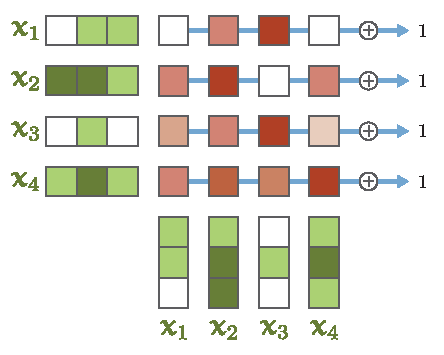
\includegraphics[width=.9\textwidth, center]{imgs/tema4/att/SAT_mtx.pdf}
    \end{column}

  \end{columns}

\end{frame}

% \begin{frame}{Ejemplo}
%   \begin{blockm}{¿Por qué funciona la attention?}
%     Supongamos que diriges un videoclub, tienes películas $\mathbf{m}$, usuarios $\mathbf{u}$, y te gustaría \textbf{recomendar} películas a tus usuarios que es probable que disfruten.
%   \end{blockm}

%   \begin{columns}
%     \begin{column}{0.4\textwidth}
%       \begin{itemize}
%         \item Necesitamos codificar cada usuario y película de forma numérica.
%         \item Podemos hacerlo de forma manual en base a los géneros.
%       \end{itemize}

%     \end{column}

%     \begin{column}{0.6\textwidth}
%       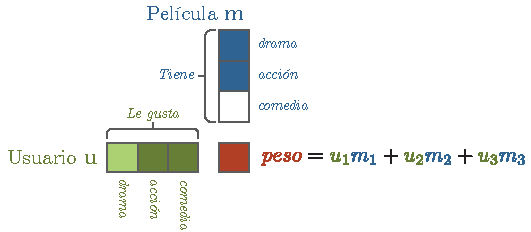
\includegraphics[width=\textwidth, center]{imgs/tema4/att/SAT_ex1.pdf}
%     \end{column}
%   \end{columns}

% \end{frame}

% \begin{frame}{Ejemplo}
%   \textbf{Importancia del signo:}\\
%   \vspace{.3cm}
%   Si $\mathbf{m}$ es romántica y a $\mathbf{u}$ le encanta el romanticismo o viceversa: \textit{Producto escalar positivo.}\\
%   Si $\mathbf{u}$ es romántica y $\mathbf{u}$ odia el romanticismo o viceversa: \textit{Producto escalar negativo.}
%   \vspace{.3cm}
  
%   \textbf{Importancia de la magnitud:}\\
%   \vspace{.3cm}
%   Las magnitudes de los géneros indican cuánto contribuye a la puntuación total.
%   \begin{itemize}
%     \item Una película puede ser un poco romántica, pero no de forma notable.
%     \item Un usuario puede no preferir el romanticismo, pero ser en gran medida ambivalente.
%   \end{itemize}

% \end{frame}

% \begin{frame}{Ejemplo}
%   Rellenar manualmente estos valores es muy costoso y prácticamente imposible cuando existen millones de películas y usuarios.\\
%   \vspace{.3cm}

%   \textbf{Para solucionarlo:}
  
%   \begin{enumerate}
%     \item Las características de cada $\mathbf{m}$ y $\mathbf{u}$ pasarán a ser parámetros del modelo.
%     \item Pedimos a los usuarios que valoren varias películas.
%     \item Optimizamos los parámetros/características para que el producto escalar coincida con la valoración.
%   \end{enumerate}

%   \begin{blockm}{Atención!}
%     Las características de cada $\mathbf{u}$ y $\mathbf{m}$ ya no representan géneros, desconocemos su significado.
%   \end{blockm}

%   A pesar de ello, estas reflejan una semántica significativa sobre el contenido de la película.

% \end{frame}

% \begin{frame}{Ejemplo}
%   Si representamos cada $m$ con 2 de las 3 nuevas características aprendidas por el modelo:\\
%   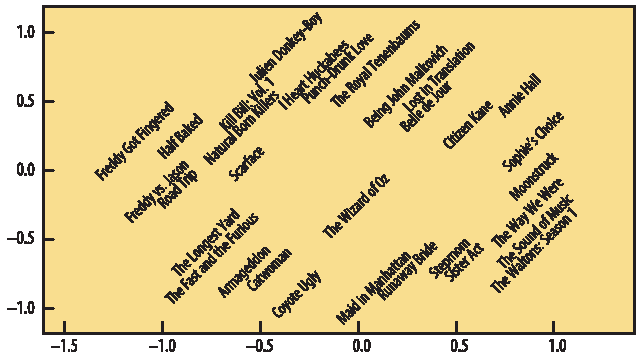
\includegraphics[width=.6\textwidth, center]{imgs/tema4/att/SAT_ex2.pdf}
%   \begin{block}{}
%     \centering
%     \textbf{El modelo es capaz de juntar películas similares sin conocer nada sobre su contenido.}
%   \end{block}
% \end{frame}

\begin{frame}{Self-attention: Ejemplo}
  % Este principio es el mismo que hace que la self-attention funcione.\\
  \vspace{.3cm}
  Imaginemos que tenemos la secuencia de palabras (frase): \textit{``El gato camina en la calle''}.\\
  \vspace{.3cm}
  \textbf{Para aplicar self-attention:}
  \begin{enumerate}
    \item Representamos cada palabra por un vector $\mathbf{x}$ (también llamado \textit{embedding}) de tamaño $k$.
    \begin{equation*}
      \mathbf{x}_{el}, \mathbf{x}_{gato}, \mathbf{x}_{camina}, \mathbf{x}_{en}, \mathbf{x}_{la}, \mathbf{x}_{calle}
    \end{equation*}
    \item Los valores de ese vector se aprenderán durante el entrenamiento. 
    \item Aplicamos self-attention a la secuencia, lo que retorna:
    \begin{equation*}
      \mathbf{y}_{el}, \mathbf{y}_{gato}, \mathbf{y}_{camina}, \mathbf{y}_{en}, \mathbf{y}_{la}, \mathbf{y}_{calle}
    \end{equation*}
    donde $\mathbf{y}_{gato}$ es la suma ponderada de todos los embeddings de la primera secuencia, ponderada por su producto escalar (normalizado) con $\mathbf{x}_{gato}$ .
  \end{enumerate}

\end{frame}

\begin{frame}{Self-attention: Ejemplo}

  \begin{blockm}{Importante}
    Como estamos aprendiendo los valores de $ \mathbf{x}_{t} $, el grado de ``relación'' entre dos palabras está \textbf{totalmente determinado por la tarea a resolver}.
  \end{blockm}

  Analizando la frase anterior, dependiendo del problema podemos esperar que, por ejemplo:

  \begin{itemize}
    \item Si creamos un modelo que detecte \textbf{artículos} en textos, los embeddings de $\mathbf{x}_{El}$ y $\mathbf{x}_{la}$:
    \begin{itemize}
      \item Tendrán un producto escalar alto respecto de las demás palabras.
    \end{itemize}
    \item Si creamos un modelo que detecte \textbf{verbos} en textos, el embedding de $\mathbf{x}_{camina}$:
    \begin{itemize}
      \item Tendrá un producto escalar alto respecto de las demás palabras.
    \end{itemize}
  \end{itemize}

\end{frame}


\begin{frame}{Self-attention: Ejemplo}

  \textbf{En resumen}:\\
  \begin{itemize}
    \item Como se ve, el producto escalar expresa cómo de ``relacionados'' están dos vectores en la secuencia de entrada.
    \item El grado de ``relación'' viene \textbf{definido por la tarea de aprendizaje}.
    \item Los vectores de salida son \textbf{sumas ponderadas} sobre toda la secuencia de entrada.
  \end{itemize}
  \vspace{.3cm}

  \textbf{¿Eso es todo?}:\\
  \begin{itemize}
    \item \textbf{No hay parámetros que aprender (por ahora):} La parte de atención no aprende ningún parámetro. La codificación de la secuencia de entrada no forma parte del mecanismo.
    \item \textbf{La entrada es un conjunto, no una secuencia:} Si alteramos el orden de las palabras, la salida será la misma, solo que también permutada. Más adelante veremos como solucionarlo.
  \end{itemize}

\end{frame}

\subsubsection{Self-attention: Mejoras}

\begin{frame}{Self-attention: Mejoras}

  \begin{block}{}
    La self-attention que se utiliza dentro de los Transformers utiliza \textbf{tres mejoras adicionales}.
  \end{block}
  \vspace{.3cm}
  \begin{enumerate}
    \item Queries, keys y values.
    \item Escalado del producto escalar.
    \item Multi-head attention.
  \end{enumerate}
  \vspace{.3cm}
  A continuación veremos cada una de ellas en detalle.

\end{frame}
\subsubsection{Self-attention: Queries, keys y values}

\begin{frame}{Self-attention: Queries, keys y values}

  \begin{blockm}{Tres representaciones}
    Cada vector $\mathbf{x}_{i}$ de la entrada se utiliza de tres formas diferentes dentro de la self-attention.
  \end{blockm}
  \begin{itemize}
    \item \textbf{Query:} Se compara con otros vectores para establecer los pesos de su propia salida $\mathbf{y}_{i}$.
    \item \textbf{Key:} Se compara con otros vectores para establecer los pesos de la j-ésima salida $\mathbf{y}_{j}$.
    \item \textbf{Value:} Se usa en el cálculo de la media ponderada que retorna el vector de salida. 
  \end{itemize}
  \vspace{.3cm}
  \begin{block}{}
    En los ejemplos que vimos hasta ahora, el vector \emph{$\mathbf{x}_{i}$ ejercía de todos estos roles a la vez}. Para facilitar la tarea a la atención, vamos a aprender \textbf{un embedding para cada rol}.
  \end{block}

\end{frame}

\begin{frame}{Self-attention: Queries, keys y values}
  Para aprender estas representaciones aplicaremos una transformación lineal al vector original.\\
  \vspace{.1cm}
  Crearemos tres matrices de tamaño $k \times k$: $\mathbf{W}_{q}, \mathbf{W}_{k}, \mathbf{W}_{v}$.\\
  \vspace{.1cm}
  Ahora, para cada elemento $\mathbf{x}_{i}$ de la secuencia de entrada tendremos \emph{tres embeddings}:
  \begin{equation*}
    \mathbf{q}_{i} = \mathbf{W}_{q}\mathbf{x}_{i} \quad \quad
    \mathbf{k}_{i} = \mathbf{W}_{k}\mathbf{x}_{i} \quad \quad
    \mathbf{v}_{i} = \mathbf{W}_{v}\mathbf{x}_{i}
  \end{equation*}

  \begin{blockm}{¿Dónde utilizarlos en self-attention?}
    \begin{equation*}
      w^{'}_{ij} = \left \langle {\mathbf{q}_{i}}^{T}, \mathbf{k}_{j} \right \rangle \quad \quad
      w_{ij} = \text{softmax}(w^{'}_{ij}) \quad \quad
      \mathbf{y}_{i} = \sum_{j} w_{ij} \mathbf{v}_{j}     
    \end{equation*}
\end{blockm}
El producto escalar se hace entre \emph{query} y \emph{key}, para la media ponderada se utilizan los \emph{values}.
\begin{block}{}
  \centering
  \textbf{Estas tres matrices serán los parámetros que aprende la self-attention.}
\end{block}
\end{frame}

\begin{frame}{Self-attention: Queries, keys y values}

  De forma gráfica:\\
  \vspace{.3cm}
  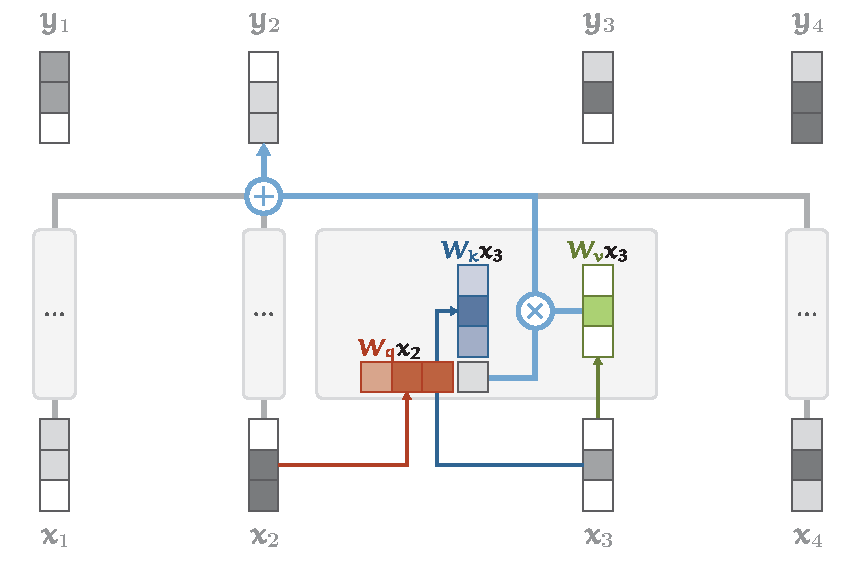
\includegraphics[width=.65\textwidth, center]{imgs/tema4/att/SAT_qkv.pdf}

\end{frame}

\subsubsection{Self-attention: Escalado del producto escalar }

\begin{frame}{Self-attention: Escalado del producto escalar }

  \begin{blockm}{Problema del softmax}
    La función softmax puede ser sensible a valores de entrada muy grandes. Estos perjudican el gradente y ralentizan o detienen el aprendizaje.
  \end{blockm}

  \begin{itemize}
    \item Aumentar el tamaño $k$ de los embeddings, aumenta el valor medio del producto escalar.
    \item Hay que reducir este valor escalando el resultado:
      \begin{equation*}
        w^{'}_{ij} = \frac{\left \langle {\mathbf{q}_{i}}^{T}, \mathbf{k}_{j} \right \rangle}{\sqrt{k}}
      \end{equation*}
  \end{itemize}

  \textbf{¿Por qué $\sqrt{k}$?}
  \begin{itemize}
    \item Dividir por la raíz cuadrada del tamaño del embedding normaliza los valores.
    \item Normalizar escala los valores evitando que unos dominen o se anulen otros.
  \end{itemize}

 \end{frame}

\subsubsection{Self-attention: Multi-head}

\begin{frame}{Self-attention: Multi-head }
  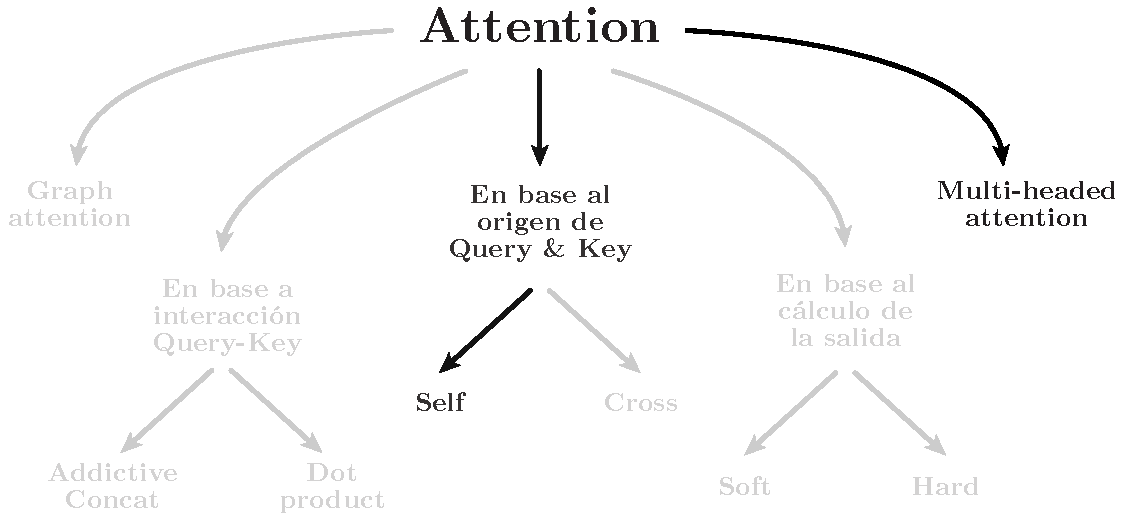
\includegraphics[width=.85\textwidth, center]{imgs/tema4/att/AttOutline multi.pdf}
\end{frame}

% \begin{frame}{Self-attention: Multi-head }


%   \begin{blockm}{Problema}
%     Una palabra puede significar cosas distintas para vecinos distintos.
%   \end{blockm}
%  \textbf{Ejemplo:} \textit{``Marta da rosas a Sara''}.\\
%   \begin{itemize}
%     \item $\mathbf{x}_{Marta}$ y $\mathbf{x}_{Sara}$ influirán en $\mathbf{x}_{da}$ en diferente cantidad, pero no de \emph{diferente forma}.
%     \item Si queremos que la información sobre quien dio las rosas y quien las recibió acabe en diferentes partes de $\mathbf{x}_{da}$ necesitamos \emph{más flexibilidad}.
%   \end{itemize}

%   \textbf{Solución:}
%   \begin{itemize}
%     \item Combinar $r$ mecanismos de self-attention para mejorar la capacidad de discriminar.
%     \item Por tanto se aprenderán $r$ matrices \emph{query}, \emph{key} y \emph{value}: $\mathbf{W}_{q}^{r}, \mathbf{W}_{k}^{r}, \mathbf{W}_{v}^{r}$.
%     \begin{block}{}
%       \centering
%       Cada uno de estos mecanismos se denomina ``cabeza'' o ``head''.
%     \end{block}
%   \end{itemize}

% \end{frame}


\begin{frame}{Self-attention: Multi-head}
  Combinar $r$ mecanismos de self-attention para mejorar la capacidad de discriminar.
  \begin{itemize}
    \item Cada uno de estos mecanismos se denomina ``cabeza'' o ``head''.
    \item Se aprenderán $r$ matrices \emph{query}, \emph{key} y \emph{value}: $\mathbf{W}_{q}^{r}, \mathbf{W}_{k}^{r}, \mathbf{W}_{v}^{r}$.
  \end{itemize}

  \begin{blockm}{Múltiples heads, múltiples salídas}
    Cada $\mathbf{x}_{i}$ produce un vector de salida $\mathbf{y}^{r}_{i}$ diferente en cada self-attention head.
  \end{blockm}
  Para obtener una salida del mismo tamaño que la entrada:
  \begin{enumerate}
    \item Concatenamos las i-ésimas salidas de cada head $\forall r$.
     \begin{itemize}
      \item Esto nos dará un vector de $r \times k$ elementos para cada entrada.
    \end{itemize}
    \item Transformamos linealmente de nuevo a tamaño $k$.
  \end{enumerate}
  \vspace{.1cm}

  \begin{block}{}
    \centering
    Necesitaremos, por tanto, una nueva matriz de pesos que denominaremos $\mathbf{W}_{o}$.
  \end{block}

\end{frame}

% \begin{frame}{Self-attention: Multi-head }

%   \begin{block}{}
%     La multi-head attention se puede ver como $r$ copias de self-attention aplicadas en paralelo.
%   \end{block}
%   \vspace{.1cm}
%   \textbf{Problema:}
%   \begin{itemize}
%     \item Cada copia tiene su propia \emph{query}, \emph{key} y \emph{value}.
%     \item Mejor rendimiento, pero $r$ veces más lento que una sola cabeza.
%   \end{itemize}
%   \vspace{.1cm}
%   Si el vector $\mathbf{x}_{i}$ tiene dimensión $k=256$ y tenemos $r=4$ heads:
%   \vspace{.1cm}
%   \begin{table}[]
%     \begin{tabular}{@{}cccc|c@{}}
%     Entrada & Proyección & q,k,v & Heads & Parámetros \\ \midrule
%     256 & 256 & 3 & 1 & 196608 \\
%     256 & 256 & 3 & 4 & 786432 \\ \bottomrule
%     \end{tabular}
%   \end{table}
% \end{frame}


% \begin{frame}{Self-attention: Multi-head eficiente}

%   \textbf{Solución:}
%   \begin{itemize}
%     \item Reducir la dimensión de las proyecciones \emph{query}, \emph{key} y \emph{value}.
%     \item Transformamos cada $\mathbf{x}_{i}$ a tamaño 64 ($256/4$) para cada \emph{query}, \emph{key} y \emph{value}.
%   \end{itemize}
%   \vspace{.1cm}

%   \begin{table}[]
%     \begin{tabular}{@{}cccc|c@{}}
%     Entrada & Proyección & q,k,v & Heads & Parámetros \\ \midrule
%     256 & 256 & 3 & 1 & 196608 \\
%     256 & 256 & 3 & 4 & 786432 \\
%     256 & 64 & 3 & 4 & 196608 \\ \bottomrule
%     \end{tabular}
%   \end{table}
%   \vspace{.3cm}
%   \begin{block}{}
%     \centering
%     Ojo, para estos ejemplos estamos omitiendo la matriz $\mathbf{W}_{o}$.
%   \end{block}
% \end{frame}

\begin{frame}{Self-attention: Multi-head}
  Finalmente, todo el proceso se puede representar como:\\
  \vspace{.5cm}
  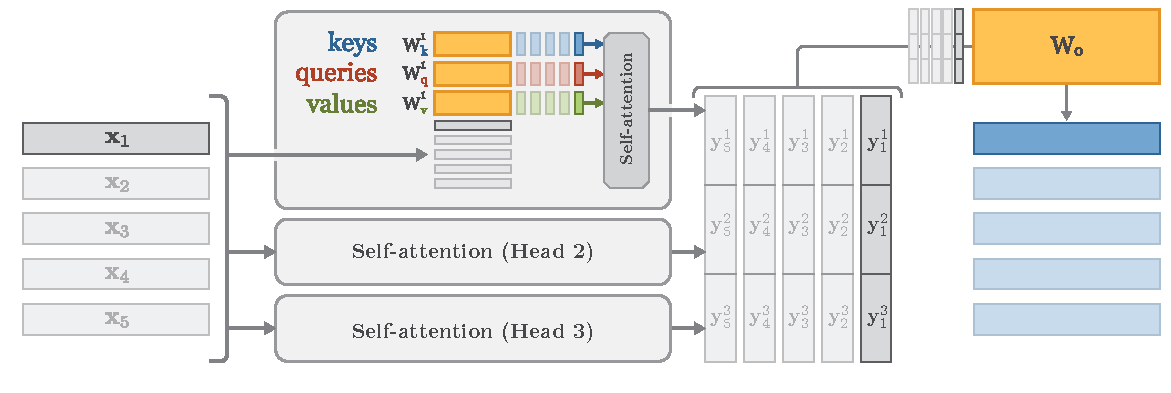
\includegraphics[width=.95\textwidth, center]{imgs/tema4/att/SAT_multihead_1.pdf}
\end{frame}

\begin{frame}{Self-attention: Multi-head}
  Finalmente, todo el proceso se puede representar como:\\
  \vspace{.5cm}
  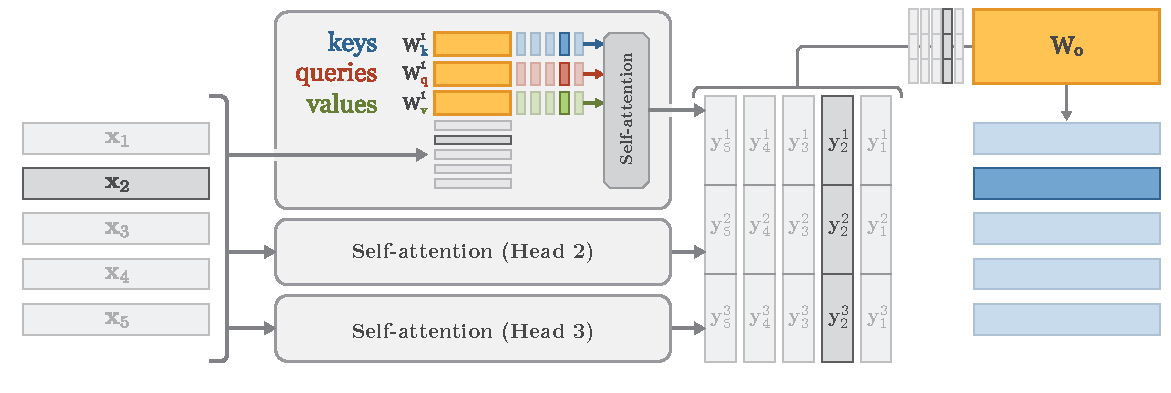
\includegraphics[width=.95\textwidth, center]{imgs/tema4/att/SAT_multihead_2.pdf}
\end{frame}

\begin{frame}{Self-attention: Multi-head}
  Finalmente, todo el proceso se puede representar como:\\
  \vspace{.5cm}
  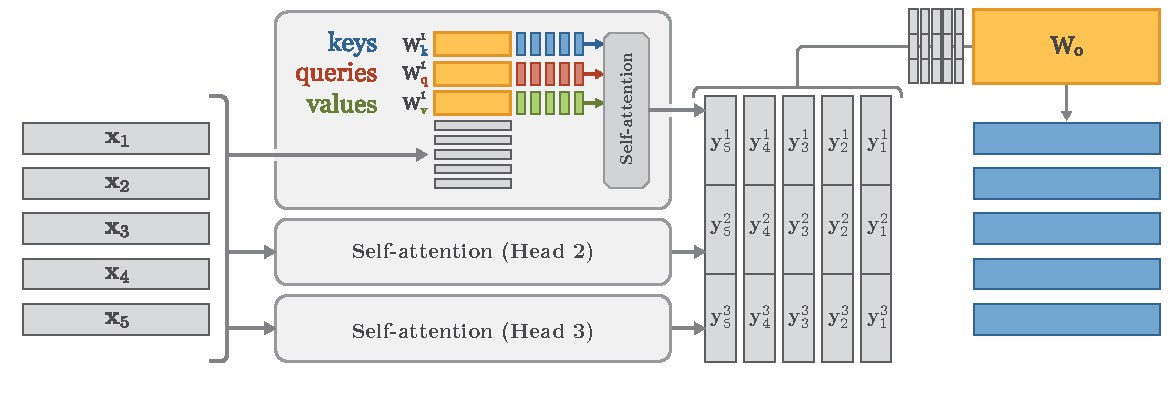
\includegraphics[width=.95\textwidth, center]{imgs/tema4/att/SAT_multihead.pdf}
\end{frame}

\subsubsection{Cross-attention}

\begin{frame}{Cross-attention}
  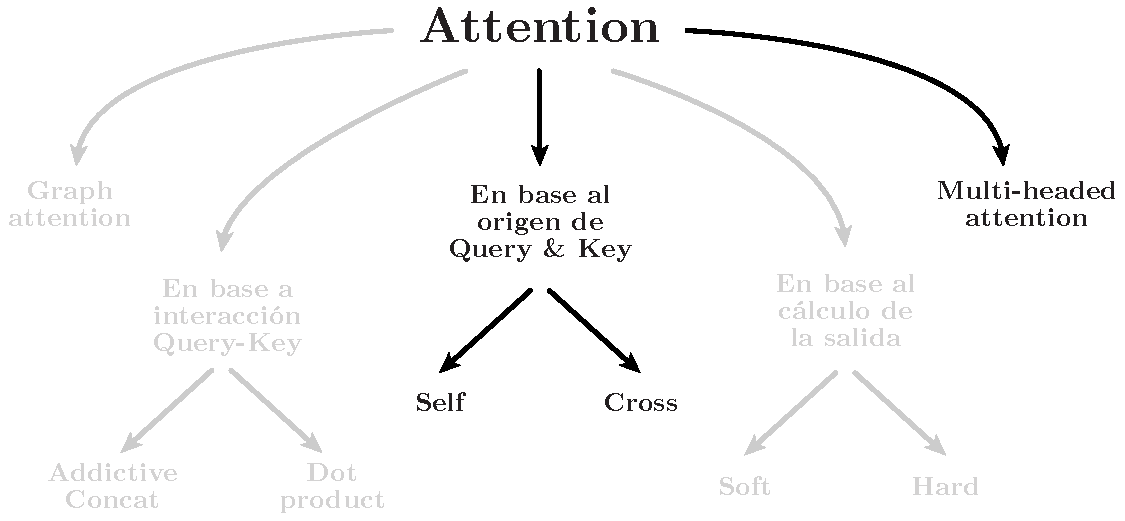
\includegraphics[width=.85\textwidth, center]{imgs/tema4/att/AttOutline cross.pdf}
\end{frame}


\begin{frame}{Self vs Cross-attention}
  
  Como se ha visto, la self-attention busca:
  \begin{itemize}
    \item La importancia de cada elemento de la secuencia para el resto de elementos de la misma.
  \end{itemize}
  \vspace{.3cm}
  \begin{block}{¿Y si el problema requiere mezclar secuencias?}
    En algún caso puede ser interesante obtener la importancia de cada elemento \textbf{de una secuencia} para \textbf{otra secuencia} diferente. Esto se conoce como \textbf{cross-attention}.
  \end{block}
  \vspace{.3cm}
  \textbf{Cambios:}
  \begin{itemize}
    \item Dos secuencias de entrada:  Una con elementos $\mathbf{x}_{i}$ y otra con $\mathbf{z}_{i}$. 
    \item Los \emph{query} se obtienen de la segunda secuencia. 
    \item Los \emph{key} y \emph{value} de la primera.
  \end{itemize}

\end{frame}

\begin{frame}{Cross-attention}

  De forma gráfica:\\
  % \vspace{.2cm}
  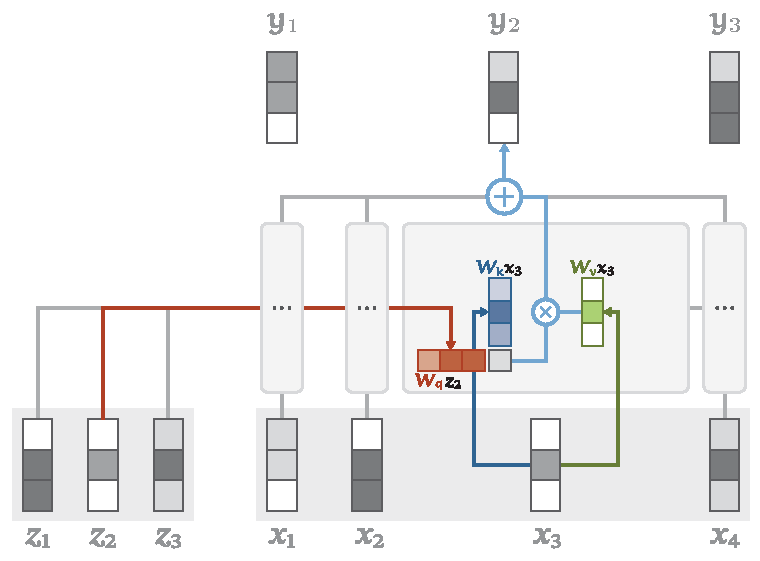
\includegraphics[width=.6\textwidth, center]{imgs/tema4/att/CAT.pdf}

\end{frame}
\begin{frame}{Cross-attention}
  
  \textbf{Aplicaciones típicas:}
  \begin{itemize}
    \item \textbf{Transformers:} Se suele ubicar en el decoder.  
    \item \textbf{Visual Question Answering (VQA):} Responder preguntas sobre imágenes:\\
    \vspace{.5cm}
    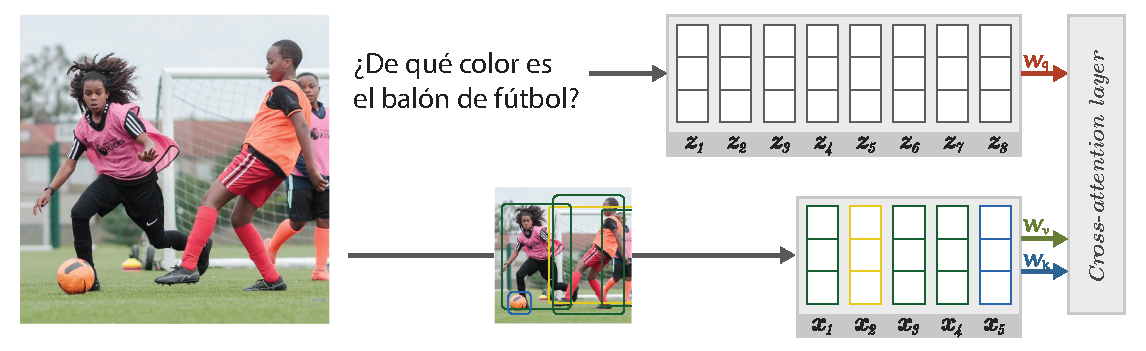
\includegraphics[width=.9\textwidth, center]{imgs/tema4/att/CAT_sample.pdf}
  \end{itemize}

\end{frame}

\begin{frame}[t]{Referencias}
  \begin{enumerate}
    \item \href{https://learningturtle.github.io/Blog/posts/attention_another_perspective_part2/}{\textbf{Attention? An Other Perspective!, Nikhil Shah}}\\
    \item \href{https://glouppe.github.io/info8010-deep-learning/?p=lecture7.md}{\textbf{Lecture 7: Attention and transformers, Prof. Gilles Louppe}}\\  
    \item \href{https://peterbloem.nl/blog/transformers}{\textbf{Transformers from scratch, Peter Bloem}}
    \item \href{https://jalammar.github.io/illustrated-transformer/}{\textbf{The Illustrated Transformer}} \\
  \end{enumerate}
\end{frame}

\end{document}
